% !TeX spellcheck = en_US
\section{EXPERIMENTS}
\label{sec:experiments}
In this section we present the results obtained with our networks. We made several experiments with the Yolo algorithm, but we don't provide a detailed list here, since it proved to be unsuitable to solve our task.\\
For the sake of comparing the results of the experiments, we divided the Kaggle training set into a test and validation set (each one is 15\% of the whole dataset) leaving the remaining 70\% of the examples for training. We then split the dataset for the classifier, consisting of all the cropped "ground truth" characters, in the same way. The examples within the test set remain the same through each execution, and the loss and accuracy metrics reported further on are computed with respect to the test set. We list the metrics for the two models separately, adding the overall Kaggle rating received over submission of the predictions for the whole test set. Submissions to the competition are evaluated on a modified version of the F1 score. To score a true positive, center point coordinates that are within the ground truth bounding box and a matching label must be provided. No other details on the metrics are provided. We used the ResNet34-encoded model for the final submission, since it was the one yielding the best results.

\subsection{Detector}
\label{ssec:detectorexp}

All models were trained using Adam optimizer using the default Keras hyper-parameters for 130 epochs. For the ResNet34 network we used a learning rate of $1 \cdot 10^{-4}$ for the first 10 epochs, decreasing it to $5 \cdot 10^{-5}$ for the next 50 epochs and using $1 \cdot 10^{-5}$ for the last 70 epochs. We used a single GPU Tesla T4 provided by Google Cloud Platform with batch size 32.\\
The same values were used for pretrained ResNet50 network except for batch size, that we set to 16 because of the deeper architecture, and for learning rate that we further lowered to $5 \cdot 10^{-6}$ after 50 epochs, since the loss function was not converging. Subsequent experiments restarting the training with lower learning rates did not improve the results.\\
The metrics shown in table \ref{tab:expdetector} suggests that, at least with the described configuration, the added complexity of the deeper architecture with pre-trained weights, resulted in worse generalization performances.

\begin{table*}[h]
	\begin{tabular}{lllllll}
		\rowcolor[HTML]{EFEFEF} 
		\textbf{Experiment}   & \textbf{Loss} & \textbf{Heatmap loss} & \textbf{Offset loss} & \textbf{Size loss} & \textbf{IoU (no tiling)} & \textbf{IoU (tiling)} \\
		ResNet34 encoder      & 1.2652        & 0.7887                & 0.3833               & 0.0932             & 0.5112                   & 0.7658                \\
		ResNet50 encoder      & 1.3792        & 0.8417                & 0.4092               & 0.1284             & 0.4067                   & 0.6760
	\end{tabular}
	\caption{Experiments with two residual architecture for detection. The first one uses ResNet34 for encoding, the second one uses the deeper ResNet50.}
	\label{tab:expdetector}
\end{table*}

\subsection{Classifier}
\label{ssec:classifierexp}

We did two experiments with the classifier, summarized in table \ref{tab:classres}. Both model were trained using Adam optimizer and batch size 1024. The first trained for 8 epochs with a learning rate of $5 \cdot 10^{-4}$ for the first 4 epochs, $1 \cdot 10^{-4}$ for the next 2 epochs, and $5 \cdot 10^{-5}$ for the following ones. The value of the learning rate was decreased manually when we noticed oscillations in the validation loss value. The second model was trained for a total of 60 epochs with learning rate $1 \cdot 10^{-5}$ and $1 \cdot 10^{-6}$ after 30 epochs. This model was trained longer, since it showed some small improvements on validation loss.\\ From the results shown, it's clear how data augmentation positively impacted the model ability to generalize.
The first one had the architecture described in figure \ref{fig:preactresblock} with preactivated residual blocks and was trained using data augmentation. The first model used an alternative architecture using standard residual blocks as already depicted in figure \ref{fig:resblock-id} and was trained without data augmentation.\\
The final submission has been done only using the first model.

\begin{table*}[h]
	%\centering
	\begin{minipage}{.7\textwidth}
	\begin{tabular}{llll}
		\rowcolor[HTML]{EFEFEF} 
		\textbf{Experiment} & \textbf{Loss} & \textbf{Accuracy} & \textbf{Kaggle score\footnote{With ResNet34-encoded model}} \\
		Augmentation + preactivation & 0.2732 & 0.9413 &  \\
		No augmentation& 0.4165 & 0.9214 &
	\end{tabular}
	\end{minipage}
	\caption{Experiments with classifier with and without data augmentation. First model is trained with preactivated residual block and data augmentation. The second one is trained with standard residual block and no augmentation.}
	\label{tab:classres}
\end{table*}

\begin{figure}[h]
	\caption{Preactivated residual block.}
	\centering
	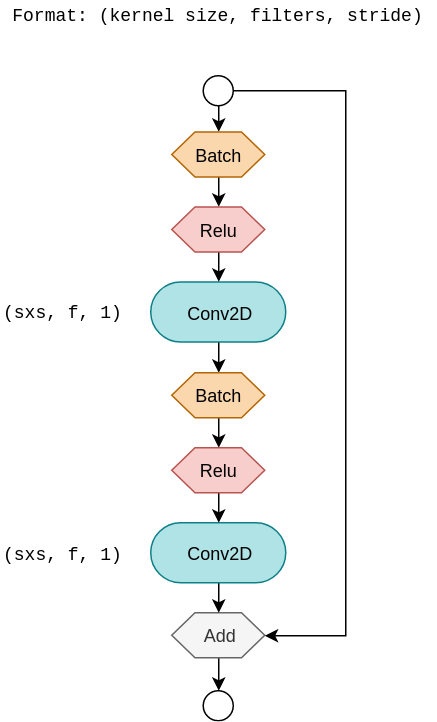
\includegraphics[width=0.35\textwidth]{architectures/resblock_pre.png}
	\label{fig:preactresblock}
\end{figure}

\section{\uppercase{Benchmarks and similar results}}
\label{sec:stateofart}

\subsection{Handwritten text recognition on historical documents}
\label{ssec:historicaldocuments}

\cite{Sanchez2019-pi} introduces four HTR (Handwritten Text Recognition) benchmarks aimed at HTR research for historical and legacy documents. These benchmarks are based on the datasets and rules previously adopted in well known open HTR competitions. The first two of these competitions (datasets ICFHR-2014, ICDAR-2015) were based on parts of the so called Bentham Papers, handwritten in English by several writers. The whole digitized collection encompasses 100000 page images of text authored by the renowned English philosopher and reformer Jeremy Bentham (1748–1832). It mainly contains legal forms and drafts in English, but also some pages are in French and Latin. Many images entail important pre-processing and layout analysis difficulties, like marginal notes, faint ink, stamps, skewed images, lines with large slope variation within the same page, slanted script, inter-line text, etc. An example of these documents is shown in figure \ref{fig:HTR_benchmark}.

\begin{figure}[h]
	\caption{An example of image from the Bentham Papers.}
	\centering
	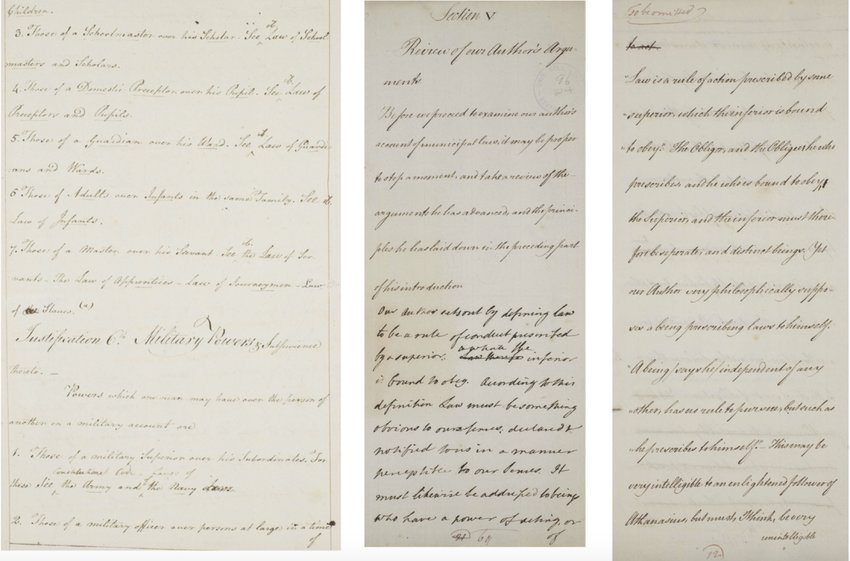
\includegraphics[width=0.45\textwidth]{various/HTR_benchmark.png}
	\label{fig:HTRbenchmark}
\end{figure}

In the third competition, the Ratsprotokolle collection (ICFHR-2016), composed of handwritten minutes of council meetings held from 1470 to 1805, was considered, while the dataset of the fourth competition was a part of the Alfred Escher Letter Collection (AEC, ICDAR-2017) which is composed of letters handwritten mainly in German but it also has pages in French and Italian. Table \ref{tab:htr-benchmarks} summarizes the baselines achieved by \cite{Sanchez2019-pi} and the best results achieved prior the publication of their paper. Note that the Word Error Rate (WER) and the Character Error Rate (CER) metrics are used. WER is defined as the minimum number of words that need to be substituted, deleted, or inserted to match the recognition output with the corresponding reference ground truth, divided by the total number of words in the reference transcripts. CER is defined in the same way but at character level.

\begin{table*}[h]
	\begin{tabular}{lcccc}
		\rowcolor[HTML]{EFEFEF}
		\cellcolor[HTML]{EFEFEF}                                     & \multicolumn{2}{l}{\cellcolor[HTML]{EFEFEF}\textbf{Best so far}} & \multicolumn{2}{l}{\cellcolor[HTML]{EFEFEF}\textbf{HTR benchmarks paper}} \\
		\rowcolor[HTML]{EFEFEF}
		\multirow{-2}{*}{\cellcolor[HTML]{EFEFEF}\textbf{Benchmark}} & CER(\%)                         & WER(\%)                        & CER(\%)                             & WER(\%)                             \\
		ICFHR-2014 Restricted                                        & 5.0                             & 14.6                           & 5.0                                 & 9.7                                 \\
		ICDAR-2015 Restricted                                        & 15.5                            & 30.2                           & 12.8                                & 30.0                                \\
		ICFHR-2016 Restricted                                        & 4.8                             & 20.9                           & 4.5                                 & 17.5                                \\
		ICDAR-2017 Traditional                                       & 7.0                             & 19.1                           & 5.8                                 & 17.6                                \\
		ICDAR-2017 Advanced                                          & 6.4                             & 16.8                           & 6.3                                 & 18.5
	\end{tabular}
	\caption{Benchmarks on handwritten text recognition from \cite{Sanchez2019-pi}.}
	\label{tab:htr-benchmarks}
\end{table*}

\subsection{Image classification on Kuzushiji-MNIST}
\label{ssec:imagemnist}

MNIST, a dataset with 70,000 labeled images of handwritten digits, has been one of the most popular datasets for image processing and classification for over twenty years. Despite its popularity, contemporary deep learning algorithms handle it easily, often surpassing an accuracy result of 99.5\%. Kuzushiji-MNIST \cite{Clanuwat2018-vm} is an alternative dataset to MNIST, more difficult than MNIST. The Kuzushiji dataset includes characters in both Kanji and Hiranaga, based on pre-processed images of characters from 35 books from the 18th century. It is constituted by three groups of data, as shown in table \ref{tab:kuzushiji-struct}. The creators of the Kuzushiji-MNIST dataset created a baseline by training a few classification algorithms and comparing them to MNIST. The best algorithm (PreActResNet-18) achieved 99.56\% on MNIST, but only 98.83\% and 97.33\% accuracy on Kuzushiji-MNIST and Kuzushiji-49 respectively, as can be seen in table \ref{tab:kuzushiji-benchmarks}.

\begin{table*}[h]
	\begin{tabular}{lllll}
		\rowcolor[HTML]{EFEFEF}
		\textbf{Dataset} & \textbf{Classes}       & \textbf{Dataset Size} & \textbf{Balanced Classes} & \textbf{Image Size} \\
		Kuzushiji-MNIST  & 10 Hiragana characters & 70.000                & Yes                       & 28x28               \\
		Kuzushiji-49     & 49 Hiragana characters & 270.912               & No                        & 28x28               \\
		Kuzushiji-Kanji  & 3832 Kanji characters  & 140.426               & No                        & 64x64
	\end{tabular}
	\caption{Description of the structure of the Kuzushiji-MNIST dataset from \cite{Clanuwat2018-vm}.}
	\label{tab:kuzushiji-struct}
\end{table*}

\begin{table*}[h]
	\begin{tabular}{lccc}
		\rowcolor[HTML]{EFEFEF}
		\textbf{Model}                            & \textbf{MNIST {[}16{]}} & \textbf{Kuzushiji-MNIST} & \textbf{Kuzushiji-49} \\
		4-Nearest Neighbour Baseline              & 97.14\%                 & 91.56\%                  & 86.01                 \\
		Keras Simple CNN Benchmark {[}4{]}        & 99.06\%                 & 95.12\%                  & 89.25\%               \\
		PreActResNet-18 {[}11{]}                  & \textbf{99.56\%}        & 97.82\%                  & 96.64\%               \\
		PreActResNet-18 + Input Mixup {[}26{]}    & 99.54\%                 & 98.41\%                  & 97.04\%               \\
		PreActResNet-18 + Manifold Mixup {[}22{]} & 99.54\%                 & \textbf{98.83\%}         & \textbf{97.33\%}
	\end{tabular}
	\caption{Benchmarks on the Kuzushiji-MNIST dataset from \cite{Clanuwat2018-vm}.}
	\label{tab:kuzushiji-benchmarks}
\end{table*}